\section{Beliefs and probabilities}
\only<presentation>{
  \begin{frame}
    \tableofcontents[ 
    currentsection, 
    hideothersubsections, 
    sectionstyle=show/shaded
    ] 
  \end{frame}
}


\only<article>{Probability can be used to describe purely chance events, as in for example quantum physics. However, it is mostly used to describe uncertain events, such as the outcome of a dice roll or a coin flip, which only appear random. In fact, one can take it even further than that, and use it to model subjective uncertainty about any arbitrary event. Although probabilities are not the only way in which we can quantify uncertainty, it is a simple enough model, and with a rich enough history in mathematics, statistics, computer science and engineering that it is the most useful.}
\begin{frame}
  \frametitle{Uncertainty}
  \begin{itemize}
  \item We cannot perfectly predict the future.
  \item We cannot know for sure what happened in the past.
  \item How can we quantify this uncertainty?
  \item Probabilities!
  \end{itemize}
  \begin{block}{Axioms of probability}
    For any probability measure\footnote{$\Sigma$ is the set of possible events, with $A \in \Sigma$ always $A \subset \Omega$. Technically $\Sigma$ is a $\sigma$-algebra} $P$ on $(\Omega, \Sigma)$,
    \begin{enumerate}
    \item<2-> The probability of the certain event is $P(\Omega) = 1$
    \item<3->The probability of the impossible event is
      $P(\emptyset) = 0$
    \item<4->The probability of any event $A \in \Sigma$ is $0 \leq P(A) \leq 1$.
    \item<5-> If $A, B$ are disjoint, i.e. $A \cap B = \emptyset$, meaning
      that they cannot happen at the same time, then
      \[
      P(A \cup B) = P(A) + P(B)
      \]
    \end{enumerate}
  \end{block}
\end{frame}

\begin{frame}
  \only<article>{ Sometimes we would like to calculate the probability
    of some event $A$ happening given that we know that some other
    event $B$ has happened. For this we need to first define the idea
    of conditional probability.  }
  \begin{definition}[Conditional probability]
    The probability of $A$ happening if we know that $B$ has happened
    is defined to be:
    \[
    P(A \mid B) \defn \frac{P(A \cap B) }{P(B)}.
  \]
\end{definition}
\only<1>{
  Conditional probabilities obey the same rules as probabilities. }
  \only<article>{
    Here, the probability measure of any event $A$ given $B$ is defined to be the probability of the intersection of of the events divided by the second event.
    We can rewrite this definition as follows, by using the definition for $P(B \mid A)$}
  \begin{block}{Bayes's theorem}
    For $P(A_1 \cup A_2)  = 1$, $A_1 \cap A_2 = \emptyset$,
    \[
      P(A_i \mid B)
      \uncover<2->{= \frac{P(B \mid A_i) P(A_i)}{P(B)}}
      \uncover<3->{= \frac{P(B \mid A_i) P(A_i)}{P(B \mid A_1) P(A_1) + P(B \mid A_2) P(A_2)}}
    \]
  \end{block}
  \uncover<4->{
  \begin{example}[probability of rain]
    What is the probability of rain given a forecast $x_1$ or $x_2$?
    \begin{columns}
      \begin{column}{0.33\textwidth}
        \begin{table}[H]
          \centering
          \begin{tabular}{c|c}
            $\outcome_1$: rain & $P(\outcome_1) = 80\%$ \\
            $\outcome_2$: dry & $P(\outcome_2) = 20\%$
          \end{tabular}
          \caption{Prior probability of rain tomorrow}
        \end{table}
      \end{column}
      
      \begin{column}{0.33\textwidth}
        \uncover<5->{
        \begin{table}[H]
          \centering
          \begin{tabular}{c|c}
            $x_1$: rain & $P(x_1 \mid \outcome_1) = 90\%$ \\
            $x_2$: dry & $P(x_2 \mid \outcome_2) = 50\%$
          \end{tabular}
          \caption{Probability the forecast is correct}
        \end{table}
        }
      \end{column}
      \uncover<6->{
      \begin{column}{0.33\textwidth}
        \begin{table}[H]
          \centering
          \begin{tabular}{c}
            $P(\outcome_1 \mid x_1) = 87.8\%$ \\
            $P(\outcome_1 \mid x_2) = 44.4\%$
          \end{tabular}
          \caption{Probability that it will rain given the forecast}
        \end{table}
        }
      \end{column}
    \end{columns}
  \end{example}
  }
\end{frame}


\begin{frame}
  \frametitle{Classification in terms of conditional probabilities}
  \only<presentation>{
    \begin{itemize}
    \item Features $x_t \in \CX$.
    \item Class label $y_t \in \CY$.
    \item Probability model $P_\model(x_t \mid y_t)$.
    \item Prior class probability $P_\model(y_t = c)$.
    \end{itemize}
  }
  \only<article>{
    Conditional probability naturally appears in classification problems. Given a new example vector of data $x_t \in \CX$, we would like to calculate the probability of different classes $c \in \CY$ given the data, $P_\model(y_t = c \mid x_t)$.  
If we somehow obtained the distribution of data $P_\model(x_t \mid y_t)$ for each possible class, as well as the prior class probability $P_\model(y_t = c)$, 
from Bayes's theorem, we see that we can obtain the probability of the class:
  }
  \[
  P_\model(y_t = c \mid x_t) = \frac{P_\model(x_t \mid y_t = c) P_\model(y_t = c)}{\sum_{c' \in \CY} P_\model(x_t \mid y_t = c') P_\model(y_t = c')}
  \]
  \only<article>{
    for any class $c$. This directly gives us a method for classifying new data, as long as we have a way to obtain $P_\model(x_t \mid y_t)$ and $P_\model(y_t)$.
  }
  \only<1>{
        \begin{tikzpicture}
          \node[RV] at (0,0) (x) {$y_t$};
          \node[RV] at (0,2) (y) {$x_t$};
          \node[RV] at (1,1) (m) {$\model$};
          \draw[->] (x) to (y);
          \draw[->] (m) to (x);
          \draw[->] (m) to (y);
        \end{tikzpicture}
      }
  \uncover<2->{
    \begin{example}[Normal distribution]
 \only<2,4>{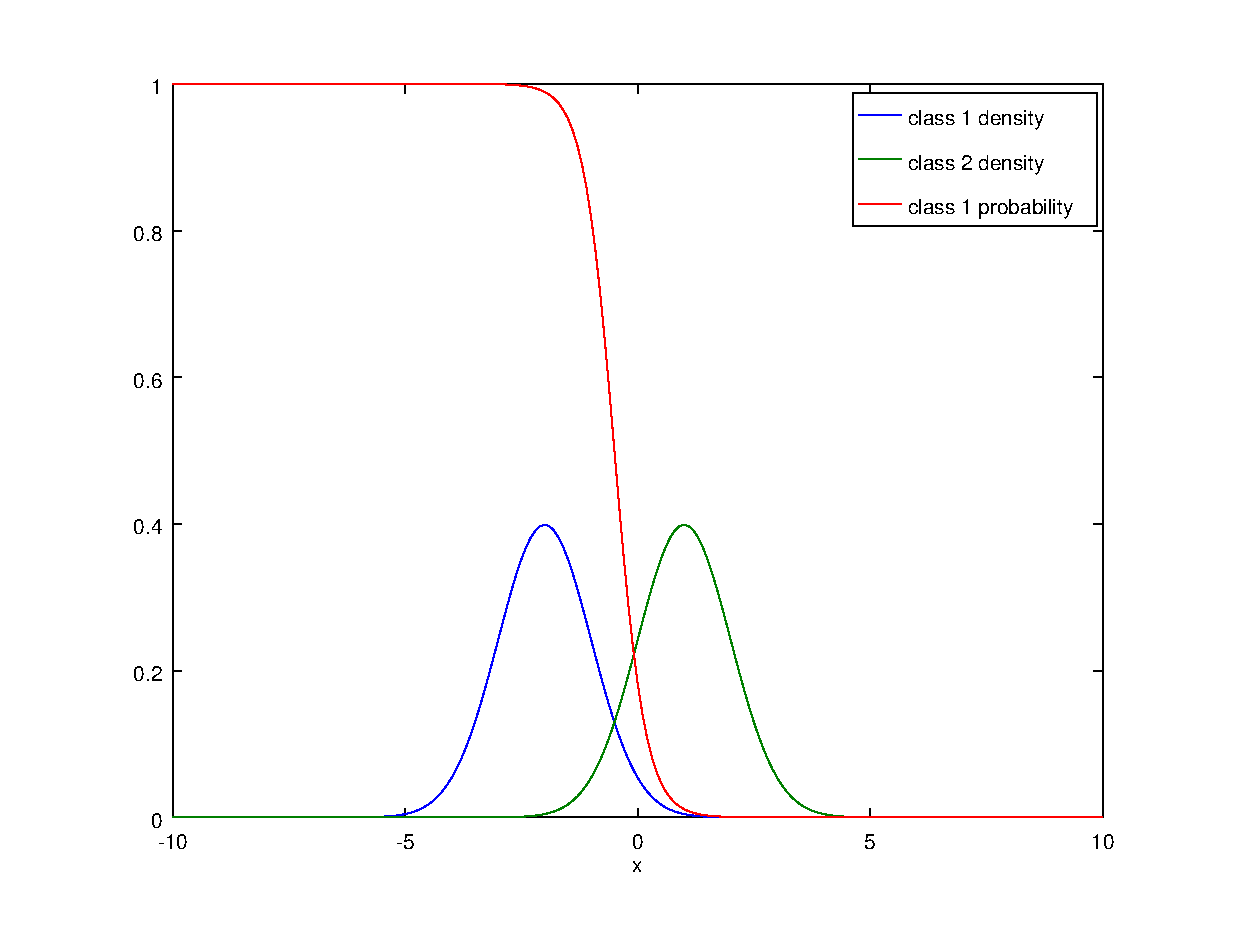
\includegraphics[width=0.5\textwidth]{../figures/equal-variance}Equal prior and variance}
      \only<3>{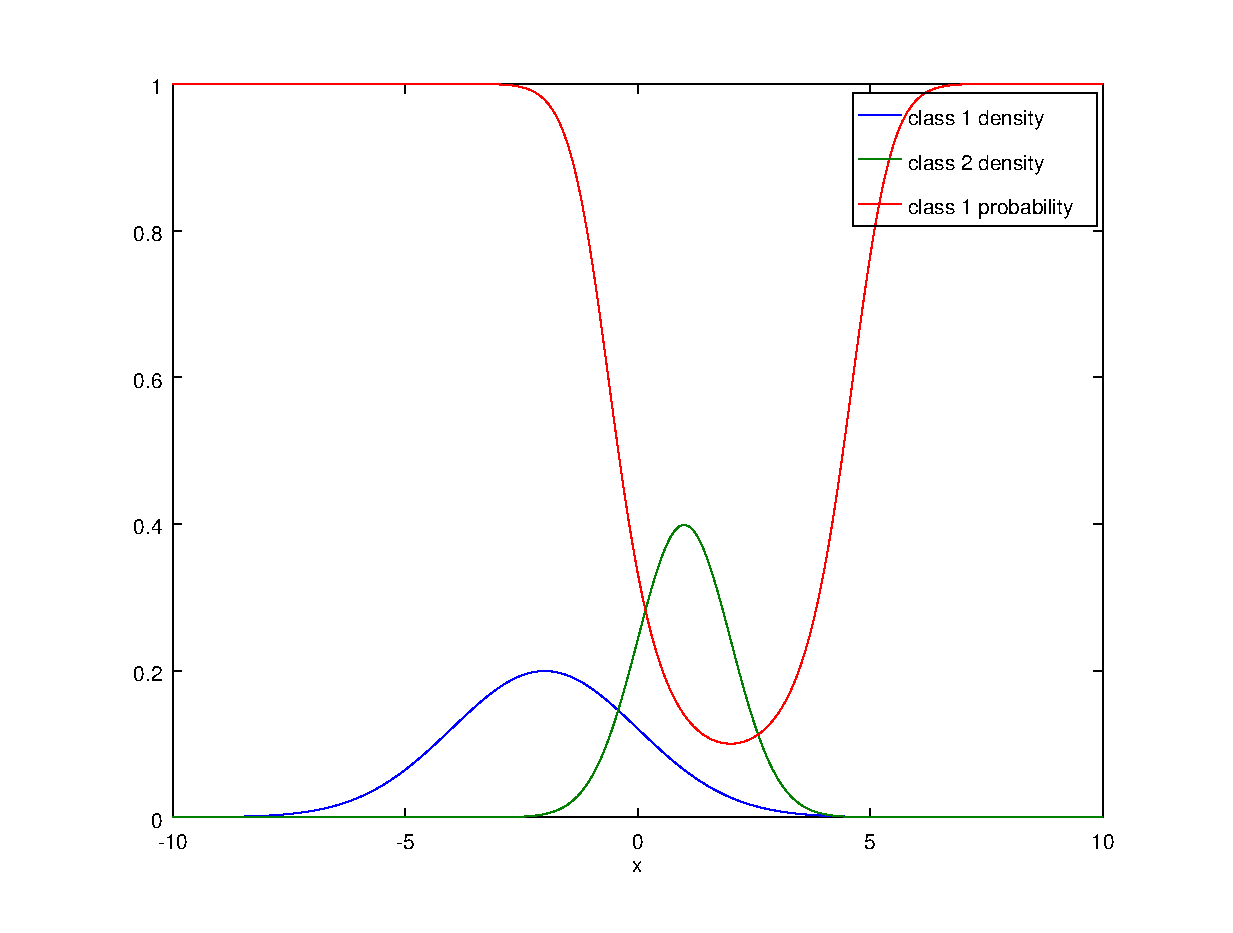
\includegraphics[width=0.5\textwidth]{../figures/unequal-variance}Unequal variance}
\only<5>{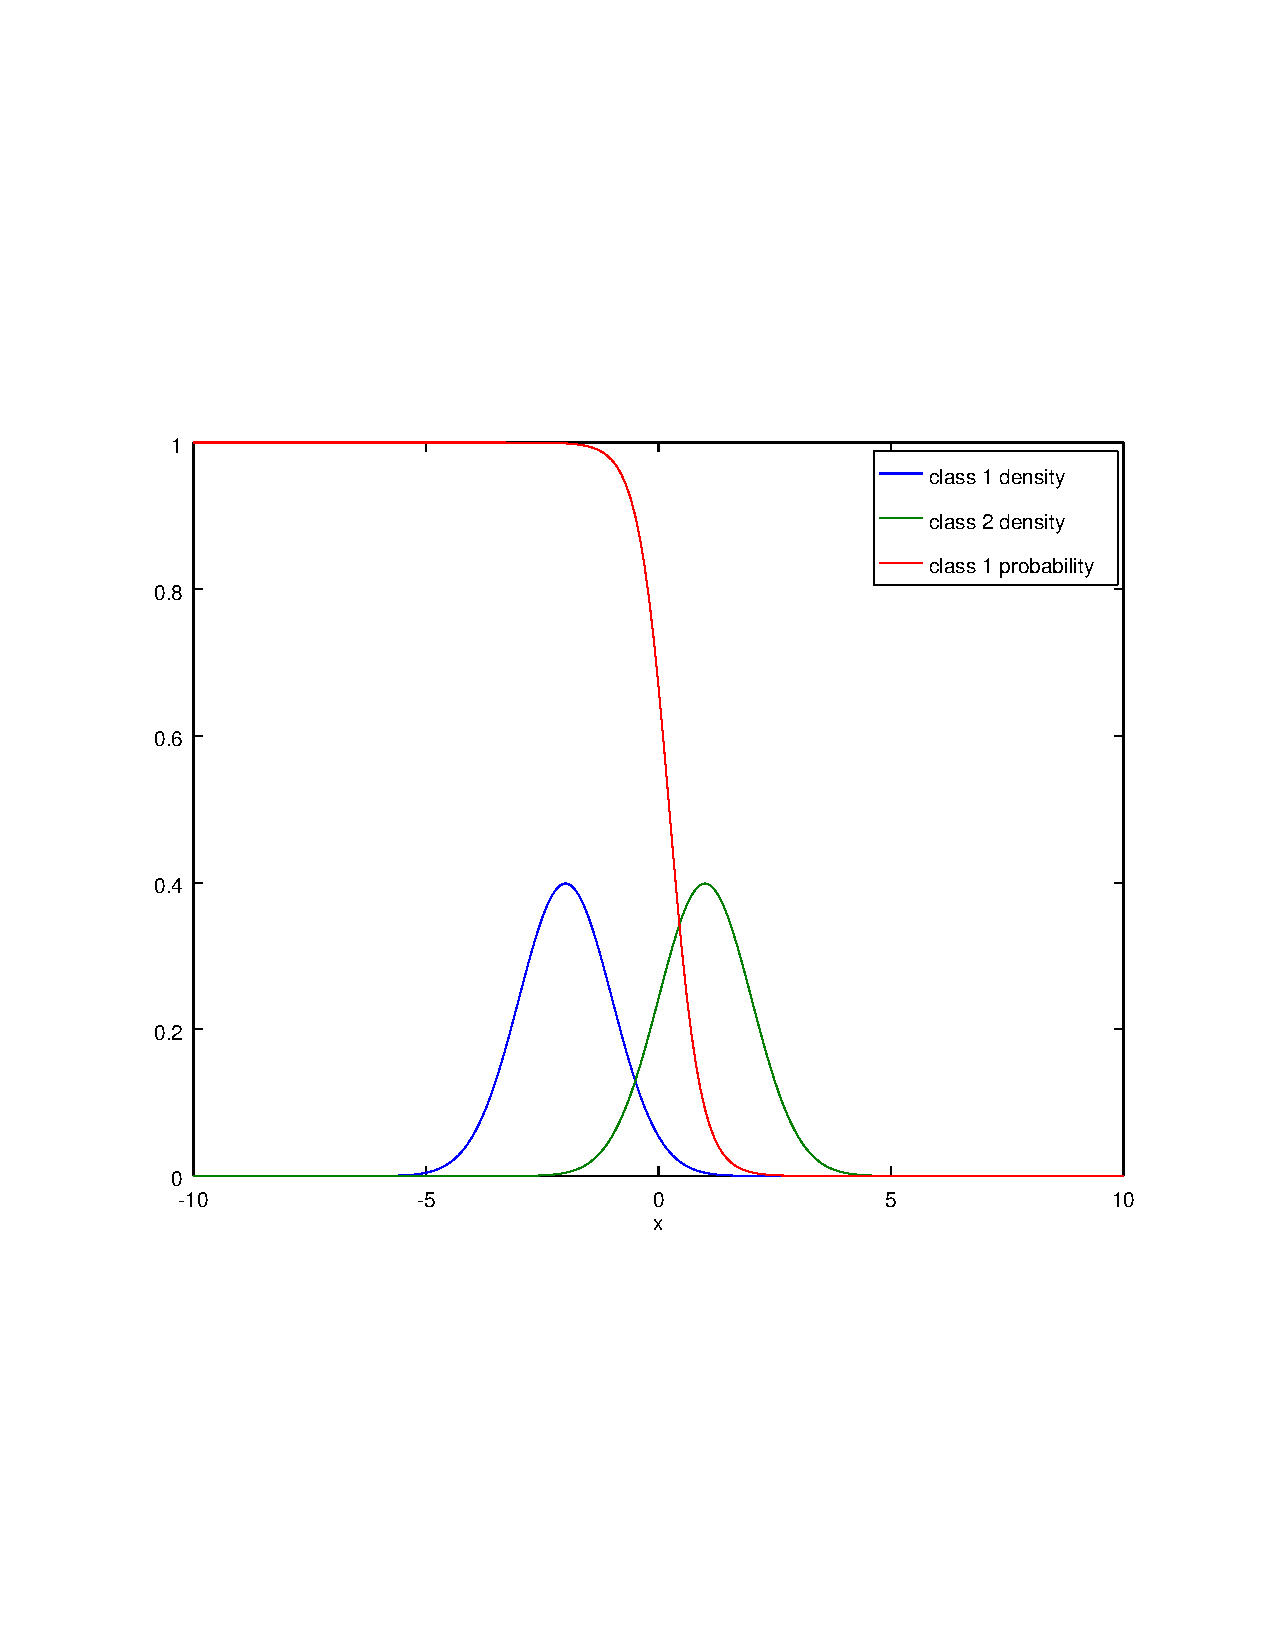
\includegraphics[width=0.5\textwidth]{../figures/unequal-prior}Unequal prior}
    \end{example}
  }
  \uncover<5>{
    \alert{But how can we get a probability model in the first place?}
  }
\end{frame}


  \begin{frame}
    \frametitle{Subjective probability}
    \only<article>{While probabilities apply to truly random events, they are also useful for representing subjective uncertainty. In this course, we will use a special symbol for subjective probability, $\bel$.}
    \begin{block}{Subjective probability measure $\bel$}
      \begin{itemize}
      \item If we think event $A$ is more likely than $B$, then $\bel(A) > \bel(B)$.
      \item Usual rules of probability apply:
        \begin{enumerate}
        \item $\bel(A) \in [0,1]$.
        \item $\bel(\emptyset) = 0$.
        \item If $A \cap B = \emptyset$, then $\bel(A \cup B) = \bel(A) + \bel(B)$.
        \end{enumerate}
      \end{itemize}
    \end{block}
  \end{frame}


  \begin{frame}
    \frametitle{Bayesian inference illustration}
    \begin{columns}
      \begin{column}{0.7\textwidth}
        \begin{block}{Use a subjective belief $\bel(\model)$ on $\Model$}
          \begin{itemize}
          \item<1-> \alert{Prior} belief $\bel(\model)$ represents our initial uncertainty.
          \item<2-> We \alert{observe history} $h$.
          \item<3->Each possible $\model$ assigns a \alert{probability} $P_\model(h)$ to $h$.
          \item<4-> We can use this to \alert{update} our belief via Bayes' theorem to obtain the \alert{posterior} belief:
            \[
            \bel(\model \mid h) \propto P_\model(h) \bel(\model)
            \tag{conclusion = evidence $\times$ prior}
            \]
          \end{itemize}
        \end{block}
      \end{column}
      \begin{column}{0.3\textwidth}
        \centering
\uncover<1->{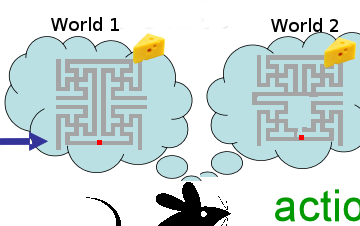
\includegraphics[width=0.5\fwidth]{../figures/rl_worlds}
          \\
          prior
        }
        \\
        \uncover<2->{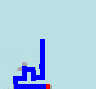
\includegraphics[width=0.5\fwidth]{../figures/rl_observations}
          \\
          evidence
        }
        \\
        \uncover<4->{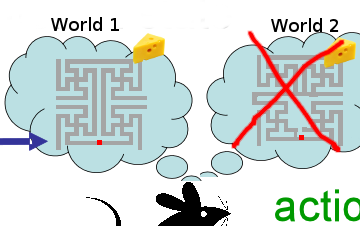
\includegraphics[width=0.5\fwidth]{../figures/rl_worlds2}
          \\ 
          conclusion
        }
      \end{column}
    \end{columns}
  \end{frame}




  \subsection{Probability and Bayesian inference}
  \only<article>{One of the most important methods in machine learning
    and statistics is that of Bayesian inference.  This is the most
    fundamental method of drawing conclusions from data and explicit
    prior assumptions. In Bayesian inference, prior assumptions are
    represented as a probabilities on a space of hypotheses. Each
    hypothesis is seen as a probabilistic model of all possible data
    that we can see.}

  \only<article>{Frequently, we want to draw conclusions from data. However, the conclusions are never solely inferred from data, but also depend on prior assumptions about reality.}




  \begin{frame}
    \frametitle{Some examples}

    \begin{example}
      John claims to be a medium. He throws a coin $n$ times and predicts its value always correctly. Should we believe that he is a medium?
      \begin{itemize}
      \item $\model_1$: John is a medium.
      \item $\model_0$: John is not a medium.
      \end{itemize}
    \end{example}
    The answer depends on what we \alert{expect} a medium to be able to do, and how likely we thought he'd be a medium in the first place.

    \only<article>{
    \begin{example}
      Traces of DNA are found at a murder scene. We perform a DNA test against a database of $10^4$ citizens registered to be living in the area. We know that the probability of a false positive (that is, the test finding a match by mistake) is $10^{-6}$. If there is a match in the database, does that mean that the citizen was at the scene of the crime?
    \end{example}
    }
  \end{frame}





  \begin{frame}
    \frametitle{Bayesian inference}
    \only<article>{
      Now let us apply this idea to our specific problem. We already have the probability of the observation for each model, but we just need to define a \emph{prior probability} for each model. Since this is usually completely subjective, we give it another symbol.
    }
    \only<article>{
      \begin{block}{Prior probability}
        The prior probability $\bel$ on a set of models $\Model$ specifies our subjective belief $\bel(\model)$ that each model is true.\footnote{More generally $\bel$ is a probability measure.}
      \end{block}
    }
    \only<article>{
      This allows us to calculate the probability of John being a medium, given the data:
      \[
      \bel(\model_1 \mid \bx) = \frac{\Pr(\bx \mid \model_1) \bel(\model_1)}{\Pr_\bel(\bx)},
      \]
      where
      \[
      \Pr_\bel(\bx) \defn \Pr(\bx \mid \model_1) \bel(\model_1) + \Pr(\bx \mid \model_0) \bel(\model_0).
      \]
      The only thing left to specify is $\bel(\model_1)$, the probability that John is a medium before seeing the data. This is our subjective prior belief that mediums exist and that John is one of them.
      More generally, we can think of Bayesian inference as follows: }
    \begin{itemize}
    \item<1-> \only<article>{We start with a set of } mutually exclusive models $\Model = \{\model_1, \ldots, \model_k\}$.
    \item<2->\only<article>{Each model $\model$ is represented by a specific probabilistic model for any possible data $x$, that is}
      \only<presentation>{Probability model for any data $x$:} $P_\model(x) \equiv \Pr(x \mid \model)$.
    \item<3-> For each model, we have a prior probability $\bel(\model)$ that it is correct.
    \item<4-> \only<article>{After observing the data, we can calculate a posterior probability that the model is correct:}
      \only<presentation>{Posterior probability}
      \[
      \bel(\model \mid x) = \frac{\Pr(x \mid \model) \bel(\model)}{\sum_{\model' \in \Model} \Pr(x \mid \model') \bel(\model')}
      = \frac{P_\model(x) \bel(\model)}{\sum_{\model' \in \Model} P_{\model'} (x) \bel(\model')}.
      \]
    \end{itemize}
    \only<5->{
      \begin{block}{Interpretation}
        \begin{itemize}
        \item $\CM$: Set of all possible models that could describe the data.
        \item $P_\model(x)$: Probability of $x$ under model $\model$.
        \item Alternative notation $\Pr(x \mid \model)$: Probability of $x$ given that model $\model$ is correct.
        \item $\bel(\model)$: Our belief, before seeing the data, that $\model$ is correct.
        \item $\bel(\model \mid x)$: Our belief, aftering seeing the data, that $\model$ is correct.
      \end{itemize}
    \end{block}
    \only<article>{It must be emphasized that $P_\model(x) = \Pr(x \mid \model)$ as they are simply two different notations for the same thing. In words the first can be seen as the probability that model $\model$ assigns to data $x$, while the second as the probability of $x$ if $\model$ is the true model.}
  }
    \only<article>{
      Combining the prior belief with evidence is key in this procedure. Our posterior belief can then be used as a new prior belief when we get more evidence.}
  \end{frame}
\begin{frame}
\begin{exercise}[Continued example for medium]
    \only<article>{ Now let us apply this idea to our specific
      problem. We first make an independence assumption. In particular, we can assume that success and failure comes from a Bernoulli distribution with a parameter depending on the model.}
    \begin{align}
    P_{\model} (x) &= \prod_{t=1}^n P_{\model} (x_t).
\tag{independence property}
    \end{align}
    \only<article>{We first need to specify how well a medium could predict. Let's assume that a true medium would be able to predict perfectly, and that a non-medium would only predict randomly. This leads to the following models:}
    \begin{align}
      P_{\model_1}(x_t = 1) &= 1, &P_{\model_1}(x_t = 0) &= 0.
                                                           \tag{true medium model}
                                                           \\
      P_{\model_0}(x_t = 1) &= 1/2, &P_{\model_0}(x_t = 0) &= 1/2.
                                                             \tag{non-medium model}
    \end{align}
    \only<article>{
      The only thing left to specify is $\bel(\model_1)$, the probability
      that John is a medium before seeing the data. This is our
      subjective prior belief that mediums exist and that John is one of
      them.}
    \uncover<3->{
      \begin{align}
        \bel(\model_0) &= 1/2,   &  \bel(\model_1) &= 1/2.
                                                     \tag{prior belief}
      \end{align}
    }
    \only<article>{Combining the prior belief with evidence is key in this
      procedure. Our posterior belief can then be used as a new prior
      belief when we get more evidence.  }
    \uncover<4>{
      \begin{align}
      \bel(\model_1 \mid x) & = \frac{P_{\model_1}(x)
        \bel(\model_1)}{\Pr_\bel(x)} \tag{posterior belief}
        \\
      \Pr_\bel(x) &\defn P_{\model_1}(x) \bel(\model_1) + P_{\model_0}(x) \bel(\model_0).
\tag{marginal distribution}
      \end{align}
    }
    Throw a coin 4 times, and have a classmate make a prediction. What your belief that your classmate is a medium? Is the prior you used reasonable?
  \end{exercise}
  \end{frame}


\begin{frame}
  \frametitle{Sequential update of beliefs}
    \only<article>{Assume you have $n$ meteorologists. At each day $t$, each meteorologist $i$ gives a probability $p_{t,\model_i}\defn P_{\model_i}(x_t = \textrm{rain})$ for rain. Consider the case of there being three meteorologists, and each one making the following prediction for the coming week. Start with a uniform prior $\bel(\model) = 1/3$ for each model.}
    {
      \begin{table}[h]
        \begin{tabular}{c|l|l|l|l|l|l|l}
          &M&T&W&T&F&S&S\\
          \hline
          CNN & 0.5 & 0.6 & 0.7 & 0.9 & 0.5 & 0.3 & 0.1\\
          SMHI & 0.3 & 0.7 & 0.8 & 0.9 & 0.5 & 0.2 & 0.1\\
          YR & 0.6 & 0.9 & 0.8 & 0.5 & 0.4 & 0.1 & 0.1\\
          \hline
          Rain? & Y & Y & Y & N & Y & N & N
        \end{tabular}
        \caption{Predictions by three different entities for the probability of rain on a particular day, along with whether or not it actually rained.}
        \label{tab:meteorologists}
      \end{table}
    }
  \begin{exercise}
    \begin{itemize}
    \item $n$ meteorological stations $\cset{\mdp_i}{i=1, \ldots,n}$
    \item The $i$-th station predicts rain $P_{\mdp_i}(y_t \mid y_1, \ldots, y_{t-1})$.
    \item Let $\bel_t(\mdp)$ be our belief at time $t$.
      Derive the next-step belief
      $\bel_{t+1}(\mdp) \defn  \bel_t(\mdp | y_{t})$ in terms of the current belief $\bel_t$.
    \item Write a python function that computes this posterior
    \end{itemize}
  \end{exercise}
  \uncover<2->{
    \[
      \bel_{t+1}(\mdp)
      \defn
      \bel_t(\mdp | y_{t})
      =
      \frac{P_\mdp(y_t \mid y_1, \ldots, y_{t-1}) \bel_t(\mdp)}
      {\sum_{\mdp'} P_{\mdp'}(y_t \mid y_1, \ldots, y_{t-1}) \bel_t(\mdp')}
    \]
  }
\end{frame}



\begin{frame}
  \frametitle{Bayesian inference for Bernoulli distributions}
  \only<1>{
    \begin{block}{Estimating a coin's bias}
      A fair coin comes heads $50\%$ of the time. 
      We want to test an unknown coin, which we think may not be completely fair. 
    \end{block}
  }
  \only<1,2>{
    \begin{figure}[h]
      \centering
      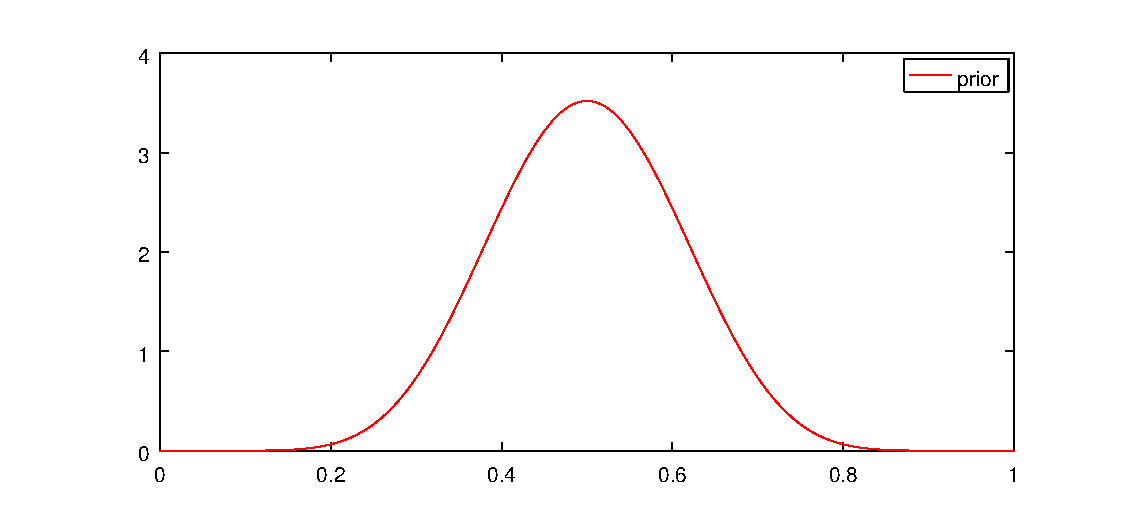
\includegraphics[width=\textwidth]{../figures/beta-prior}
      \caption{Prior belief $\bel$ about the coin bias $\theta$.}
    \end{figure}
  }
  \only<2>{
    For a sequence of throws $x_t \in \{0,1\}$,
    \[
    P_\theta(x) \propto \prod_t \theta^{x_t} (1 - \theta)^{1 - x_t}
    = \theta^{\textrm{\#Heads}} (1 - \theta)^{\textrm{\#Tails}}
    \]
  }
  \only<3>{
    \begin{figure}[h]
      \centering
      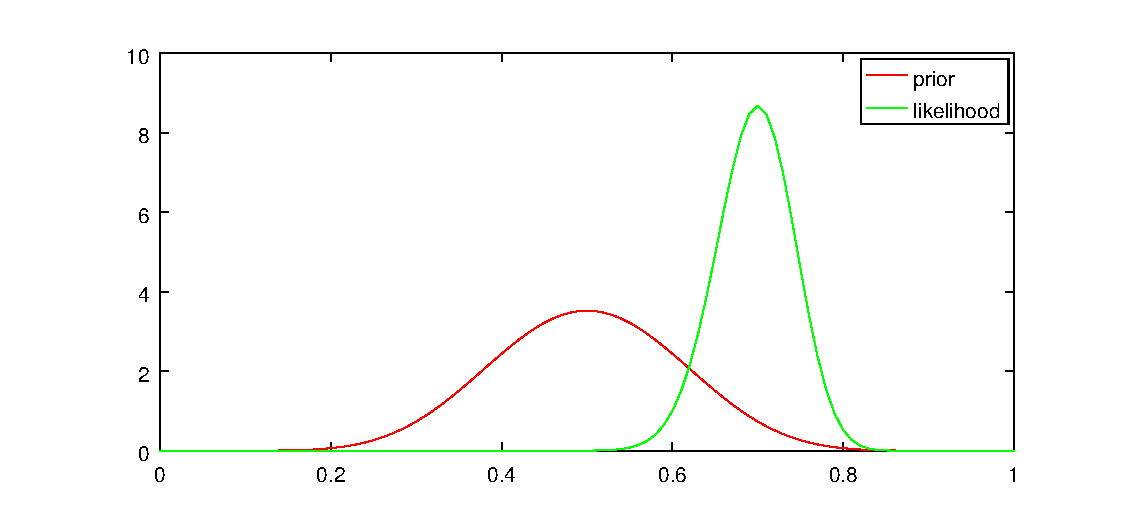
\includegraphics[width=\textwidth]{../figures/beta-likelihood}
      \caption{Prior belief $\bel$ about the coin bias $\theta$ and likelihood of $\theta$ for the data.}
    \end{figure}
    Say we throw the coin 100 times and obtain 70 heads. Then we plot the \alert{likelihood} $P_\theta(x)$ of different models.
  }
  \only<4>{
    \begin{figure}[h]
      \centering
      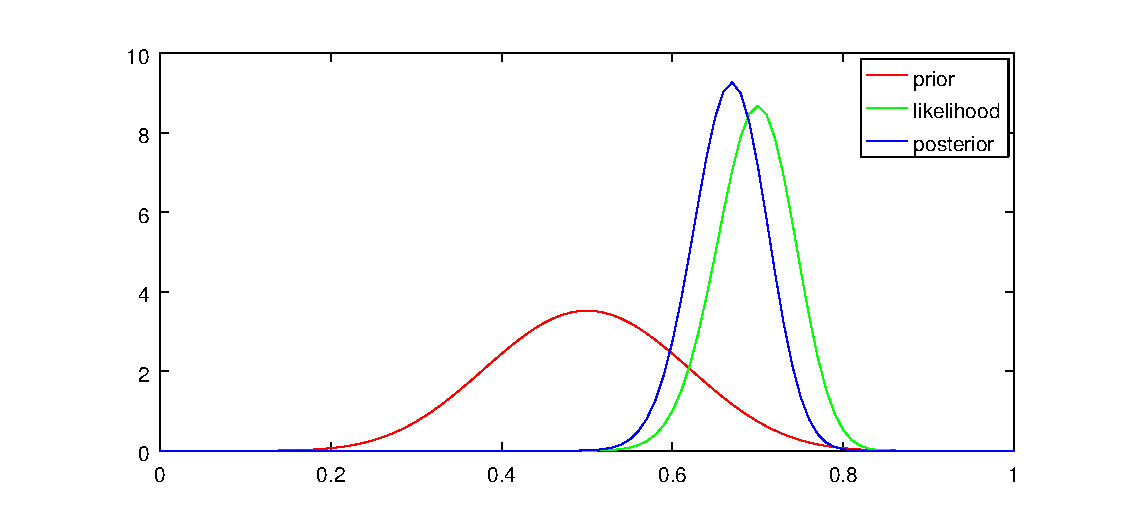
\includegraphics[width=\textwidth]{../figures/beta-posterior}
      \caption{Prior belief $\bel(\theta)$ about the coin bias $\theta$, likelihood of $\theta$ for the data, and posterior belief $\bel(\theta \mid x)$}
    \end{figure}
    From these, we calculate a \alert{posterior} distribution over the correct models. This represents our conclusion given our prior and the data.
  }
\end{frame}



  %%% Local Variables:
  %%% mode: latex
  %%% TeX-engine: xetex
  %%% TeX-master: "notes.tex"
  %%% End:
